\documentclass[12pt,UTF8]{ctexbook}
\usepackage{ctex}
\usepackage{array}
\usepackage{graphicx}
\usepackage{wrapfig}
\usepackage[table,dvipsnames]{xcolor}
\usepackage{tabularx}
\usepackage{amsmath}
\usepackage{amssymb}
\usepackage{xfrac}
\usepackage{eucal}
\usepackage{titlesec}
\usepackage{amsthm}
\usepackage{tikz-cd}
\usepackage{enumitem}
\usepackage{verbatim}
\usepackage{fontspec,xunicode,xltxtra}
\usepackage{xeCJK} 

\definecolor{gl}{RGB}{246, 252, 240}
\definecolor{gd}{RGB}{236, 244, 230}
\definecolor{bg}{RGB}{242, 244, 228}


\setCJKmainfont[BoldFont=STZhongsong]{STSong}
\setCJKmonofont{simkai.ttf} % for \texttt
\setCJKsansfont{simfang.ttf} % for \textsf
\setlength\parskip{8pt}
\setlength{\fboxsep}{12pt}
\renewcommand\thesection{\arabic{chapter}.\arabic{section}}
\newtheorem{df}{定义}[section] 
\newtheorem{pp}{命题}[section]
\newtheorem{ex}{例子}[section]
\newtheorem{sk}{思考}[section]
\newtheorem*{so}{解答}
\newenvironment{proof2}{\paragraph{\textbf{证明:}}}{\hfill$\square$}
\newtheorem{xt}{习题}[section]
\newtheorem{cor}{推论}[pp]
% 列举环境的行间距
\setenumerate[1]{itemsep=0pt,partopsep=0pt,parsep=0pt,topsep=0pt}
\setitemize[1]{itemsep=0pt,partopsep=0pt,parsep=0pt,topsep=0pt}
\setdescription{itemsep=0pt,partopsep=0pt,parsep=0pt,topsep=0pt}
% 章节字体大小
\titleformat{\section}{\zihao{-2}\bfseries}{ \thesection }{16pt}{}
% 封面
\title{\zihao{0} \bfseries 第一册}
\author{\zihao{2} \texttt{大青花鱼}}
% \date{\bfseries\today}
\date{}
% 正文
\begin{document}
\maketitle
\tableofcontents
\newpage

\chapter{从自然数到有理数}

\section{分数、整数、有理数}
我们已经学过自然数:$0,1,2,3,\cdots$。自然数是$0$和$1$相加得到的数。
从$0$开始,不断加$1$,就能得到任何自然数。
自然数之间做加法和乘法,得到的还是自然数。

加法和乘法都满足结合律和交换律,乘法满足对加法的分配律。

自然数是自然产生的。当人们发现两头牛和两天有共同之处时,自然数的概念就诞生了。

为了回答类似“三个人分七只鸡”的问题,人们发明了除法。除法是乘法的逆运算。除法产生了分数。自然数可以看作分母是$1$的分数。
分数之间可以做加法、乘法和除法,得到的还是分数。

为了回答类似“五个鸡蛋吃了两个还剩几个”的问题,人们发明了减法。减法是加法的逆运算。
比如,$3+2=5$,于是$3=5 - 2$。

既然可以写出$5-2$,那么可不可以写$0-2$呢?$0-2$有什么含义呢?

借用“五个鸡蛋吃了两个还剩几个”的思路,$0-2$可以表示“本没有鸡蛋,借来两个鸡蛋吃了两个还剩几个”。
这里剩下的,是“欠两个鸡蛋”,是一种负债状态。因此,这样的数称为\textbf{负数}。

我们一般把$0-2$中的$0$去掉,只记为$-2$。$-2$满足$-2+2=0$。对某个数,比如$73$来说,$73+(-2)=73+(0-2)=73-2$。
也就是说,一个数加上$-2$,就和减去$2$一样。以此类推,可以得到:
$$ -1, -2, -3, \cdots $$
它们由$1,2,3,\cdots$前加上减号得到,表示$0$减去$1,2,3,\cdots$的结果,读作“负一”、“负二”、“负三”等等。
我们把负数带的减号称为\textbf{负号}(读作“负”),和一般减法区别开来。

一般来说,在任何分数前加上负号,也可以得到一个负数,表示$0$减去它的结果。

有没有$-0$呢?$-0$就是$0-0$,也就是$0$自己,所以就没有必要加负号了。

自然数和它们的负数合称\textbf{整数}。我们把$-1, -2, -3, \cdots$这些负数称为\textbf{负整数},
把原来$1,2,3,\cdots$这些数称为\textbf{正整数},和负整数相对。由于$-0$就是$0$,约定$0$既不是正数,也不是负数。
于是整数分为正整数、负整数和$0$。

分数和它们的负数合称\textbf{有理数},我们把带负号的分数称为\textbf{负有理数}或\textbf{负分数},
把原来的分数(除了$0$)称为\textbf{正有理数}或\textbf{正分数}。
正有理数包括正整数,负有理数也包括负整数,有理数包括整数。

自然数或分数前面加负号得到的负数,叫做它的\textbf{相反数}。反过来,一个负整数或负数去掉负号得到的数,也叫做这个它的相反数。
约定$0$的相反数就是$0$。于是,每个有理数都有唯一的相反数。除了$0$以外,相反数总是成对的。一个有理数的相反数的相反数,就是它自己。

\begin{sk}\label{sk:0-0-0}
    一个有理数前面加上负号,一定会得到一个负数吗?
\end{sk}

加上一个负数,就和减去它的相反数一样。所以,现实问题中遇到和加法对应的具体概念,都可以用减法和负数表示相反或相对的概念。
比如,如果把“往东走三步”视作“$+3$”,那么“往西走两步”就可以视作“$-2$”。“原地往东走三步,再往西走两步”,就可以视作
“$0+3-2$”。计算得到$1$,就表示最终和原来比,往东走了一步。

\section{有理数的大小}
加法不仅可以表达累加的概念,还可以用于比较大小。比如,$5$比$3$大,可以理解为$5$是$3$再加自然数$2$得到的,
而$3$却没法通过$5$加上一个自然数得到。一般来说,两个不同的自然数或分数,如果其中一个加上某个自然数或分数等于另一个,
那么它比另一个数小,另一个数比它大。

用这个方法,我们可以比较有理数的大小。首先,任何负有理数加上它的相反数都得到$0$,
所以$0$大于任何负有理数。而任何正有理数都大于$0$,所以任何正有理数大于任何负有理数。

我们约定大于$0$的数叫做\textbf{正数},小于$0$的数叫做\textbf{负数}。正整数、正有理数都是正数,负整数、负有理数都是负数。
这样的约定和前面负数的定义是一致的。

负有理数之间如何比较大小呢?举例来说,$0 = -3 + 3 = -3 + 1 + 2$,所以$-3 + 1 = 0 - 2 = -2$。
$-2$由$-3$加上自然数$1$得到,所以$-3$小于$-2$。进一步分析,我们发现,自然数$1$来源于“$3$可以写成$1+2$”。
所以我们可以总结出两个负有理数比较大小的方法:看它们的相反数。相反数中较大的,可以写成较小数加上一个分数,
于是,相反数较大的负有理数加上这个分数,就等于相反数较小的负有理数。因此,相反数较大的负有理数比较小,
相反数较小的负有理数比较大。

正数和负数可以比较大小。所以,现实问题中涉及到相反或相对的概念比较大小时,可以用有理数表示。
比如,今天延安的气温是$3.4$摄氏度,长春的气温是$-8.2$摄氏度,哈尔滨的气温是$-15.1$摄氏度,那么延安气温最高,
长春气温比延安低,而哈尔滨气温又比长春低。

\section{数轴}
为了直观表示有理数,我们引入\textbf{数轴}的概念。

从左往右画一条直线,在中间取一点表示$0$,称为\textbf{原点}。选择适当长度作为单位长度,规定右边是\textbf{正方向},
往右移动一个单位长度就是“$+1$”,那么,从原点出发,每隔单位长度取一个点,就可以表示出$1,2,3\cdots$。
相对的,往左移动一个单位长度就是“$-1$”,类似可以表示出$-1,-2,-3\cdots$。这就是数轴。

数轴上的点,越往右就越大,越往左就越小。正数都在$0$右边,负数都在$0$左边。
两个数比较大小,可以在数轴上找到对应的点:靠右的比较大,靠左的比较小。

数轴上的数还可以做加减法。在数轴上找到一个数$a$的位置,然后往右移动$b$个单位长度,就得到了$a+b$。
反之,往左移动$b$个单位长度,就得到了$a-b$。

数轴上的相反数:$3$是从原点往右移动$3$个单位长度到达的点,而$-3$是从原点往左移动$3$个单位长度到达的点。如果先往右移动$3$个单位长度,
再往左移动$3$个单位长度,就会回到原点。一般来说,在数轴上先往右再往左(或先往左再往右)走一样多的单位长度,
最终自然就回到原点。这说明任何数加上自己的相反数,都得到$0$。

\begin{sk}\label{sk:0-1-0}
    有理数在数轴上吗?怎么在数轴上找到一个有理数?
\end{sk}

\section{乘方}
乘法可以更方便地表示若干个相同的数相加。比如,我们用$3 \times 4$表示$3+3+3+3$。
那么,能不能方便地表示若干个相同的数相乘呢?

我们把$3\times 3$称为$3$乘$2$\textbf{次方},把$7\times 7\times 7\times 7\times 7$称为$7$乘$5$次方。

同一个数连乘几次,叫做它乘几次方。连乘的结果,叫做它的几\textbf{次方}或几\textbf{次幂}。这种运算叫做\textbf{乘方}或\textbf{乘幂}。

我们把$7$的$5$次方记作$7^5$,把$7$称为\textbf{底数},把$5$称为\textbf{指数}。
这样记法,比$7\times 7\times 7\times 7\times 7$更方便。

一个数的$1$次方就是它自己。一个数的$2$次方也叫做它的\textbf{平方}。一个数的$3$次方也叫做它的\textbf{立方}。

约定任何数的$0$次方是$1$。

$7\times 7\times 7\times 7\times 7 = (7\times 7\times 7)\times (7\times 7)$。
用乘方表示这个关系,就是:$7^5 = 7^3 \times 7^2$。注意到$5 = 3 + 2$。
用日常的话来说,$5$个$7$相乘,等于$3$个$7$相乘,再和$2$个$7$相乘。

同底数乘方的积,等于指数之和的乘方。乘方的乘法,可以转化为指数的加法。
因此,乘方的除法,也可以转化为指数的减法。

比如,$7^{5-2} = 7^3 = 7^5 \div 7^2$。

既然乘方的乘除可以转化为指数的加减,那么是否有负指数?能否定义一个数的负数次方?

如果定义$7^{-3}$为:$7^{-3} \times 7^3 = 7^{0} = 1$,那么
$7^{(-3)}$就等于$\frac{1}{7^3}$。一个数的负几次方,就是$1$除以它的几次方。

显然,$0$没有负数次方。

\begin{sk}\label{sk:0-2-0}
    \mbox{}\\
    1. 约定任何数的$0$次方是$1$,有什么好处?\\
    2. 负数次方和前面负数的定义矛盾吗?
\end{sk}

\chapter{从变量到方程(上)}

\section{数和代数}
讨论数的性质时,我们常常发现,总结一些普遍的规律,需要用很多话来说清楚。比如:
\begin{ex}\label{ex:1-0-0}
    \mbox{} \\ 
    \indent $4 = 3 + 1,\,\,\, 4^2 - 3^2 = 4 + 3.$ \\
    \indent $5 = 4 + 1, \,\,\,5^2 - 4^2 = 5 + 4.$\\
    \mbox{}\\
    \indent $(2 \times 4 + 1)^2 = 8 \times 10 + 1.$\\
    \indent $(2 \times 5 + 1)^2 = 8 \times 15 + 1.$
\end{ex}
我们想总结两个对所有数都适用的规律,但只举了几个例子。这种方法不好。

有没有更好的方法呢?

对于第一个规律,我们可以说:如果天元比地元大$1$,那么天元的平方减去地元的平方等于天元加地元。
对于第二个规律,我们可以说,每个自然数两倍加$1$的平方除以$8$余$1$。

我们用“天元”、“地元”、“每个自然数”代替了具体的$4$和$5$,以说明这是更普遍的规律,
而不是只对$4$和$5$成立的等式。这种思想叫做\textbf{代数}的思想。
代数可以让我们暂时忽略具体的数,把重点放在数与数之间的关系上。我们能轻松看出这些关系是普遍的,不依赖特定的数。
我们把这样的关系叫做\textbf{代数关系}。

为了和数区别,“天元”、“地元”、“每个自然数”等称为\textbf{量}。量是对可以运算的概念的称呼。
量可以有现实意义,比如物理学里会讨论物理量,也可以没有现实意义,比如数学中代替数的量可以称为数量。

在讨论问题的时候,如果我们认为一个量代替的数不会变化,就说这个量是\textbf{常量};如果会变化,就说它是\textbf{变量}。

我们可以变量描述上面两个规律:
$$ \mbox{如果天} = \mbox{地}+1, \,\,\,\mbox{那么}\mbox{天}^2 - \mbox{地}^2 = \mbox{天} + \mbox{地}. $$
$$  (2\times \mbox{甲} + 1)^2 \,\mbox{除以} \,8\,\mbox{余}\,1.$$
为了方便,我们一般用字母命名的变量来指代数。
$$ \mbox{如果} a = b+1, \,\,\,\mbox{那么} a^2 - b^2 = a + b. $$
$$  (2\times x + 1)^2 \mbox{除以} 8\mbox{余} 1.$$
其中变量$a,b,x$可以变成$3,4,5$或任何一个自然数。

\textbf{用变量代替数,可以用简明的语言揭示更复杂、更普遍的规律。}

\begin{sk}\label{sk:1-0-0}
    \mbox{}\\
    1. 用代数的方法,说一说怎样比较两个负有理数的大小。\\
    2. 用代数的方法,定义一个数的负数次方。\\
    3. 用代数的方法,描述加法结合律、加法交换律、乘法结合律、乘法交换律和分配律。
\end{sk}

\section{代数式}
含有变量的算式叫做\textbf{代数式}。为了区别,我们把只有数的算式叫做\textbf{数式}。

$a + 2$,$1.84\times x - 3$,$0.79 j^2 - \frac{h+1}{n} + 5 $等等都是代数式。

数式既表示计算过程,也表示计算的结果:一个数。把数式中的数用变量代替,我们不再计算结果,只关心计算过程本身。
这对我们找出并解释计算过程中的规律很有帮助。掌握了计算的规律后,我们再用具体的数代替变量(称为\textbf{取值}或\textbf{代入}),
就能更快更好地算出结果。

乘号$\times$和$x$或$X$很像,为了避免混淆,一般省略乘号,或用$\cdot$代替乘号。
$1.84\times x - 3$可以写成$1.84 x - 3$或$1.84\cdot x - 3$

代数式中不同的变量称为\textbf{元}。只与一个变量有关的式子叫做\textbf{一元式},
和多个变量有关的式子叫做\textbf{多元式}。

变量和数通过四则运算得到的代数式,叫做\textbf{有理式}。
变量和数通过加法、减法和乘法得到的代数式,叫做\textbf{整式}。
如果除法中涉及了变量,就叫\textbf{分式}。有理式中除了整式,就是分式。
\begin{ex}\label{ex:1-1-0}
    \mbox{} \\
    \indent 整式:$x^3 + 5x - 3.32$,$a + b^2 - 2C$,$(b - 4)^9.$ \\
    \indent 分式:$\frac{1 - 0.9r + v^2}{3B - k}$,$n^2 - 7 + \frac{0.88}{(H - 6)^3}$, $t - (t + 0.382g)^{-3}.$\\
\end{ex}

我们知道,数的乘法比加减法优先。比如,计算$4 + 3\times 6$时,我们要先计算$3\times 6 = 18$,再计算$4 + 18 = 22$。
先计算加法是不对的。代数式特别是整式中,我们也更关心乘法。我们把变量和数相乘的部分称为\textbf{项}。$0.54xba$,$-1.24\cdot gb\cdot 1.19 \cdot g^2$,$u\cdot 98K$
各是一项,$10b - V$是两项的差。

项是变量和数的乘积。变量之间不一定能运算,但数与数之间可以运算。我们可以把项中所有的数相乘,放在最前面,叫做项的\textbf{系数}。
其次,同一个变量多次相乘,可以放在一起,作为连乘,用乘方表示。这样得到更简洁清晰的项。
代数式某一项化简后,总是一个数乘以若干个变量的乘幂。

如果某一项是另一项乘以某个(不是零的)数,就说它们是\textbf{同类项}。同类项的变量部分相同,因此根据乘法分配律,可以合并,规则是把系数相加。
比如,$3.52x^2y$可以和$0.19x^2y$合并,得到$3.71x^2y$。\textbf{合并同类项}也是代数式化简的一部分。

一项中所有变量的指数的和,叫做它的\textbf{次数}。比如$3.71x^2y$的次数是$3$,它可以叫$3$次项。
不含变量部分的项叫\textbf{常数项}。常数项次数为$0$。

整式是变量和数通过加减法和乘法得到的代数式。由于乘法优先计算,可以认为整式是一些项做加减法得到的。
合并同类项后,如果只剩下一项,就说它是\textbf{单项式}。一般来说剩下不止一项,称为\textbf{多项式}。
多项式的每一项都是单项式。多项式次数最高的项叫做最高次项。最高次项的次数就叫多项式的次数。
如果多项式每一项次数都相等,就称它为\textbf{齐次多项式}。
\begin{xt}\label{xt:1-0-0}
    \mbox{} \\
    1. 合并同类项:\begin{itemize}
        \item $3 + 9x^3 + 5x - 7x^3 - 3.32 - 1.05x$
        \item $ab^2 + (c-b)a^2 - ba(b - c) + c(b + a)c + (a - c)b(c + a) - (b + c)bc.$
    \end{itemize}
    2. 判断是否是齐次多项式:\begin{itemize}
        \item $\frac{(a+b)^3}{a - b}$
        \item $a^4 - bx^3$
        \item $a^4b^4\left(\frac{a^2}{b} + \frac{c^2}{a}\right)^4$
    \end{itemize}
\end{xt}

\section{等式和方程}
\textbf{等式}就是把两个式子或多个式子用等号连起来。\textbf{不等式}就是把两个式子或多个式子用不等号连起来。
一般情况,默认是两个式子。

等式可以是真的,也可以是假的。前者也叫等式成立,后者也叫等式不成立。

按大小关系,\textbf{不等号}分为两类:大于类和小于类。按是否包含相等关系,不等号分为两类:严格类和可等于类。
一共有四个不等号:“$<$”(严格小于),“$\leqslant$”(小于等于),“$>$”(严格大于),“$\geqslant$”(大于等于)。

等式的基本性质:两边同时加、减、乘、除同一个量,成立的等式仍然成立。

为了解决生活中的问题,我们学过简单的方程。把未知的数,用变量表示。问题中的相等关系,就变成了含变量的等式,
称为\textbf{方程}。解决这个问题,求出变量的值,称为\textbf{解方程}。变量的值称为\textbf{方程的解}。

如果问题中的条件是不等关系,我们就得到了含变量的\textbf{不等式}。解决这个问题,求出变量的值,
称为\textbf{解不等式}。变量的值称为\textbf{不等式的解}。

\chapter{集合和映射}
\section{集合}
我们用集合表示一类事物。把不同性质的事物聚集在一起,合起来考虑,就是\textbf{集合},简称\textbf{集}。
构成集合的事物称为集合的\textbf{元素}。
\begin{enumerate}
    \item 集合的元素互不相同。
    \item 集合的元素没有顺序。
    \item 集合的元素是确定的:一个事物要么属于该集合,要么不属于。
\end{enumerate}

某个事物$a$属于集合$A$,记作$a\in A$。某个事物$a$不属于集合$A$,记作$a\notin A$。

\begin{ex}\label{ex:2-0-0}
    \mbox{} \\ 
    \indent 可以在大括号中列出集合的元素,比如:$\{1,2,3\}$是一个集合,$\{1,2,2,3\}$不是集合。 \\
    \indent 也可以在大括号中用条件描述集合。集合的元素是满足条件的元素,比如:$\{ a | a\mbox{是偶数}\}$。竖线左边是元素的样子,右边是它满足的条件。\\
    \indent 还可以直接用文字描述集合,比如:一年的十二个月份是一个集合。\\
    \indent 除了以上方式,也可以用示意图、图表、列表等方式表示集合。
\end{ex}

没有元素的集合称为\textbf{空集},记为$\varnothing$。

自然数、整数、分数、有理数都是集合。自然数一般简记为$\mathbb{N}$,分数一般简记为$\mathbb{F}$,
整数一般简记为$\mathbb{Z}$,有理数一般简记为$\mathbb{Q}$。“$a$是自然数”可以记为$a\in\mathbb{N}$。

如果集合$A$的元素都是集合$B$的元素,就说$A$是$B$的\textbf{子集},记为$A\subseteq B$,
$B$是$A$的\textbf{母集},记为$B\supseteq A$。
如果两者不相同,就说$A$是$B$的\textbf{真子集},记为$A\subset B$,$B$是$A$的\textbf{真母集},
记为$B\supset A$。

如果$A$是$B$的子集,那么$B$中不属于$A$的元素也构成一个集合,称为$A$在$B$中的\textbf{补集},记为$B\backslash A$。
讨论问题的时候,我们可能会默认某个集合是问题涉及的所有事物的集合,其他集合都是它的子集。这样的集合一般称为\textbf{全集}。
全集存在的时候,集合$A$在全集中的补集可以简称为$A$的补集,记为$\bar{A}$或$A^c$。

自然数集、整数集、分数集和有理数集有以下关系:
\begin{align}
    \mathbb{N}\subset\mathbb{Z}\subset\mathbb{Q} \notag \\
    \mathbb{N}\subset\mathbb{F}\subset\mathbb{Q} \notag
\end{align}
以上每个集合中的正数与负数,构成它的子集,一般用上标$+$和$-$标示。比如,$\mathbb{Z}^+$就表示正整数集合,$\mathbb{Q}^-$就表示负有理数集合。

考虑若干个集合。由属于其中至少一个集合的元素构成的集合,称为这些集合的\textbf{并集};
由属于所有集合的元素构成的集合,称为这些集合的\textbf{交集}。
两个集合$A, B$的并集记为$A\cup B$,交集记为$A\cap B$。

几个集合交集为空集,就说它们\textbf{不相交}。几个集合中任取两个,都不相交,就说它们两两不相交。
如果集合$A$的一些子集两两不相交,而且它们的并集是$A$,就说这些集合是$A$的\textbf{分划}。

\section{判断和集合}
判断和集合有密切的关系。把一个判断涉及的个体看作全集,使判断为真的个体就是全集的一个子集,使判断为假的个体就是它的补集。
比如“自然数$n$能被$3$整除”这个判断,涉及了自然数这个全集。使它为真的自然数构成自然数集的子集,使它为假的自然数的集合是前者的补集。

全判断和有判断,也包含了集合的概念。比如,“所有兔子的眼睛都是红的”这个判断中,“所有兔子”可能指世界上所有的兔子,
也可能指说话的人面前的几只兔子,因此是含混不清的。只有当我们把兔子的集合确定下来,比如“贵州毕节市黔西县境内的兔子”,
这个判断才是清楚无疑的。同样地,“至少有一个学生得了满分”这个判断,也要在明确了学生的集合,比如“
黎阳小学$2020$级三班的全体学生”,才是有意义的。

数学中,也有各种判断。为了方便,我们引进两个符号:$\forall$和$\exists$。$\forall$表示“任一”、“每个”,
$\exists$表示“存在”、“至少有一个”。对某个集合$A$中元素的全判断,可以写成$\forall x \in A, \, P(x)$;
对某个集合$A$中元素的有判断,可以写成$\exists x \in A, \, P(x)$。其中$P(x)$表示一个包含变量$x$的判断。

比如,“所有$10$的倍数,个位数都是$0$”可以写成:$\forall x \in \mathbb{N}$,$ 10 x$的个位数是$0$。
“至少有一个一位数比$5$大”可以写成:$\exists x \in [0,\ldots ,9], \, x > 5$。

\begin{wrapfigure}{r}{0.42\textwidth} %this figure will be at the right
    \flushright
    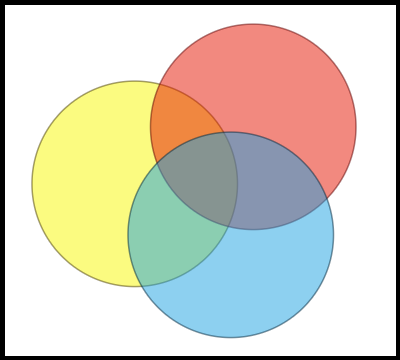
\includegraphics[width=0.4\textwidth]{叠圈图0.png}
\end{wrapfigure}

复合判断也可以用集合的方式表达。

为了更好理解,我们可以用\textbf{叠圈图}直观理解集合的关系。

如右图,每个圈表示一个集合,圈内的区域表示属于该集合的元素,圈外的区域表示不属于该集合的元素,也就是该集合(关于全集的)补集。
两个圈重叠的部分就表示同时属于两者的元素的集合,也就是两个集合的交集。而两个圈各自的部分加上重叠的部分,
就是至少属于其中之一的元素的集合,也就是两个集合的并集。

叠圈图可以让我们直接看到集合之间的关系。

联言判断是多个判断的全判断。使各个判断为真的个体都构成一个集合$S_i$,因此,通过这些集合的集合$I$,
可以给出使联言判断为真的个体对应的集合:
$$ \{x \,| \,\forall i \in I, x \in S_i \} $$
这个集合是各个集合$S_i$的交集,我们将它记为:$ \bigcap_{i\in I} S_i. $

或言判断是多个判断的有判断。因此,使或言判断为真的个体对应的集合:
$$ \{x \,|\, \exists i \in I, x \in S_i \} $$
这个集合是各个集合$S_i$的并集,我们将它记为:$ \bigcup_{i\in I} S_i. $

\begin{wrapfigure}{r}{0.42\textwidth} %this figure will be at the right
    \flushright
    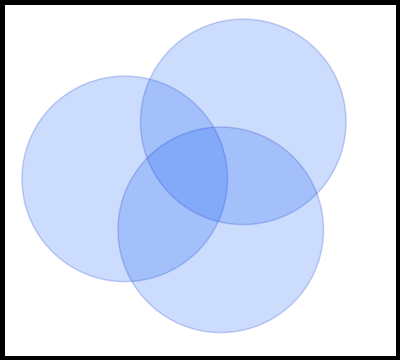
\includegraphics[width=0.4\textwidth]{叠圈图1.png}
\end{wrapfigure}

右图中,联言判断对应着所有圈交叠的区域(颜色最深的部分),而或言判断对应着所有蓝色的区域的总和。

\begin{xt}\label{xt:2-0-0}
    验证集合满足以下性质:
    \begin{itemize}
        \item $A \cup B = B \cup A$
        \item $A \cap B = B \cap A$
        \item $A \cup A = A \cap A = A$
        \item $A \cap (B \cap C) = (A \cap B) \cap C$
        \item $A \cup (B \cup C) = (A \cup B) \cup C$
        \item $A \cap \varnothing = \varnothing$
        \item 如果$A \subseteq B$,那么$A \cap B = A$,$A \cup B = B$
        \item $(A \cap B) \cup (A \cap C) = A \cap (B \cup C)$
        \item $(A \cup B) \cap (A \cup C) = A \cup (B \cap C)$
    \end{itemize}  
\end{xt}

\begin{sk}\label{sk:2-0-1}
     有个理发师,坚持只给那些不给自己理发的人理发。那么,他是否该给自己理发呢?
\end{sk}

\section{映射}
我们用\textbf{映射}表示事物之间的对应关系。把一个事物对应到另一个事物,可以理解为事物的变换或对事物进行操作。
因此映射也叫做\textbf{变换}或\textbf{操作}。\textbf{函数}是把数量对应到数量的映射。

我们把映射涉及的事物用两个集合记录:\textbf{出发集}和\textbf{到达集}。映射把出发集的一个元素对应到到达集的一个元素。
用变量$x$指代出发集的元素,$x$的取值在出发集里变化时,映射对应的元素也在到达集里变化,可以用变量$y$表示。
一般称$x$为\textbf{自变量},$y$为\textbf{应变量}。

如果把映射记作$f$,那么可以用$y = f(x)$或$f:x\mapsto y$表达“映射把出发集的元素和到达集的元素对应起来”这件事。

出发集中,某个映射涉及的元素集合称为映射的\textbf{定义域};
到达集里,某个映射涉及的元素集合则称为映射的\textbf{值域}。定义域是出发集的子集,值域是到达集的子集。

需要强调的是,映射可以把多个元素对应到同一个元素,但不会把一个元素对应到多个元素。

每个一元式都可以用来定义映射。比如,设定定义域是自然数集$\mathbb{N}$后,
代数式$4-0.3x+9x^2+\frac{(1-x+2.69x^4)}{0.5x-1.385}$就可以定义映射:
$$ \forall x\in\mathbb{N}, \quad x \mapsto 4-0.3x+9x^2+\frac{(1-x+2.69x^4)}{0.5x-1.385}. $$
这里我们把映射的定义域设为自然数集:$\mathbb{N}$。
如果把定义域设成另一个集合,比如$\{1,2,3\}$或全体偶数,就定义了另一个映射。

确定了定义域后,每个含有变量的判断也可以定义一个映射。比如,设定定义域是$\{1,2,5,6\}$后,“$3n+1$能被$5$整除”就可以定义映射:
$$ \forall n\in \{1,2,5,6\} , \quad n \mapsto 3n+1\,\mbox{能被}\,5\,\mbox{整除。} $$

\begin{sk}\label{sk:2-0-2}
    全判断$\forall x \in A, \, P(x)$和映射$\forall x\in A, \, x \mapsto P(x)$之间存在什么关系?
\end{sk}

\chapter{有理数的运算}
我们已经学过自然数和分数的运算。两个自然数可以做加法、减法和乘法,任两个分数可以做加法、减法、乘法和(不为零的)除法。
把自然数、分数扩展到有理数后,两个有理数可以做加法、减法、乘法和不为零的除法。

有理数的运算和自然数、分数相比,多了与负数有关的运算。为了讨论方便,我们首先介绍一个表示负数的方法:
每个负数都能表示成$-a$的形式,其中$a$是它的相反数,是一个正数。

\section{有理数的加减法}
我们先来看与负数有关的加减法。按照负数的定义,任何负数$-a = 0 - a$。所以,一个数加上一个负数,就等于减去它的相反数:
$$ b + (-a) = b + (0 - a) = b - a$$
换句话说,一个数减去一个正数,就等于加上它的相反数。另一方面,一个数减去一个负数,也等于加上它的相反数:
$$ b - (-a) = b - (0 - a) = b + a$$
两者可以用同一句话描述:\textbf{减去一个数,等于加上它的相反数。}

于是,有理数的减法总可以转化为有理数的加法。

再来看两个有理数的加法。如果两者都是正数,就是我们熟悉的分数加法。
如果被加数是正数,加数是负数,那么和等于被加数减加数的相反数:
$$ b + (-a) = b - a$$
式子中$a$和$b$都是正数。如果$b > a$,那么和是正数。如果$b < a$,和是负数,它的相反数是:
$$ -(b - a) = 0 - (b - a) = a - b$$
因此和是$a - b$的相反数。\\
如果被加数是负数,加数是正数,那么和等于加数减被加数的相反数:
$$ (-a) + b = 0 - a + b = b - a$$
式子中$a$和$b$都是正数。类似地,如果$b > a$,那么和是正数。如果$b < a$,和是负数,相反数是$a - b$。
如果两者都是负数,和也是负数:
$$ (-a) + (-b) = 0 - a + (0 - b) = 0 - a - b$$
这个和加上$a + b$等于$0$,因此,和是$a + b$的相反数。

看得出,上面讨论中$a$和$b$以及它们的大小关系很重要。为了方便总结,我们引进\textbf{绝对值}的概念:
\begin{df}\label{df:3-0-0}
    正数的\textbf{绝对值}是它自身,负数的绝对值是它的相反数。$0$的绝对值是$0$。
\end{df}
按照这个定义,可以把前面讨论的结果简化:

如果两个有理数同为正数(负数),那么它们的和也是正数(负数),绝对值是它们绝对值的和。如果两个有理数一正一负,那么
它们的和的正负与两者绝对值较大者的正负一致,和的绝对值是绝对值较大者减去绝对值较小者的差。

总结两个有理数的加减法:
\begin{center}
    \fbox{
        \shortstack[l]{
            1. 将减法转为加法。\\
            2. 任何数与$0$相加都得到自身。\\
            3. 计算两个数的绝对值。\\
            4. 如果两个数同正负,取绝对值的和,加上对应的正负号。\\
            5. 如果两个数一正一负,用较大的绝对值减去较小的绝对值,\\
            加上绝对值较大的数的正负号。
        }
    }
\end{center}

\begin{xt}\label{xt:3-0-0}
    算一算:\\
    \indent $2.56 - (-1.9)$,$(-4) + 3.29$,$10.8 + (-42.15).$ \\
    \indent $-59.76 + 40.3$,$-2.8 - 6.6$,$-5.09 - (-2.9).$ \\
    \indent $-1.76 -(-5.21) - 1.874$,$3.202 - (-1.94) - 1.57$,$2 + (-9.18) - (20.354).$ \\
    \indent $3 - 2 - (-8) + (-2.2)$,$-8.1 - ((-1.6) - 1.96 + (-3.9 + 1.203)).$
\end{xt}

\section{有理数的乘除法}
讨论有理数的乘除法,可以从最简单的情况开始:$(-1) \times 1$和$(-1) \times (-1)$。按照定义,
$$(-1) \times 1 = (0 - 1) \times 1 = 0 \times 1 - 1 \times 1 = 0 - 1 = -1.$$
同理,$(-1) \times 0 = 0$,于是:
\begin{align}
    (-1) \times (-1) &= (-1) \times (0 - 1) \notag \\
    &= (-1) \times 0 - (-1) \times 1 \notag \\
    &= 0 - (-1) = 1. \notag
\end{align}
类似的还有$1 \times (-1) = 1$以及$0 \times (-1) = 0$。所以,$-1$的乘法性质可以归纳为“负零得零,负正得负,负负得正”。

同理,把乘数换成一般的数,也有:
$$(-1) \times a =  0 - a = -a, \quad (-1) \times (-a) = (-1) \times (0 - a) = a.$$
也就是说,一个数乘以$-1$,总得到它的相反数。任何负数都等于它的绝对值乘以$-1$。

因此,两个有理数相乘,乘积的绝对值总是两者绝对值的乘积,只需把$-1$作为因子提出来,然后看$-1$的个数确定乘积的正负就可以了。
如果两个数都是正数,那么不需要考虑$-1$的问题。如果两者一正一负,那么有一个$-1$,乘积是负数,
如果两个数都是负数,有两个$-1$,“负负得正”,于是乘积是正数。

如果乘数或被乘数是$0$,结果是$0$。

除法是乘法的逆运算,我们只需要把涉及负数的除法转为乘法即可。

除数是正有理数$a$的时候,除以$a$等于乘以它的倒数:$\frac{1}{a}$。

除数是负有理数$-a$的时候,我们要找到$b \div (-a)$,也就是使得$c \times (-a) = b$的数$c$。
根据前面对乘法的推导,$ b \times (-1) \times \frac{1}{a} = c \times a \times \frac{1}{a} = c$,或者说
$$c = b\times \left((-1) \times \frac{1}{a}\right)$$
其中的关键是说明$(-a)$存在倒数:$-\frac{1}{a}$。
$$ (-a)\times \left(-\frac{1}{a}\right) = (-a)\times \left((-1) \times \frac{1}{a}\right) = a \times \frac{1}{a} = 1. $$
所以无论除数是正有理数还是负有理数,\textbf{除以一个数,等于乘以它的倒数。}

于是,有理数的除法总可以转化为有理数的乘法。

综上所述,可以这样总结有理数的乘除法:
\begin{center}
    \fbox{
        \shortstack[l]{
            1. 将除法转为乘法。\\
            2. 任何数与$0$相乘都得到$0$。\\
            3. 计算两个数的绝对值。\\
            4. 如果两个数同正负,取绝对值的乘积。\\
            5. 如果两个数一正一负,取绝对值乘积的相反数。
        }
    }
\end{center}

\begin{xt}\label{xt:3-0-1}
    \mbox{}\\
    \indent 算一算:\\
    \indent $4.51 \times (-2.2)$,$(-1.2) \times (-3.9)$,$(-1.8)\times 0.8.$ \\
    \indent $1.98 \div (-0.3)$,$-2.8 \div (-0.7)$,$5.2 \div (3 \div (-1.5))$, $(-3) \div (0.5 \times (-2.4)).$ \\
    \indent 思考:\\
    \indent 1. 为什么“任何数与$0$相加都得到自身”?\\
    \indent 2. 为什么“任何数与$0$相乘都得到$0$”?\\
    \indent 3. 为什么说“涉及负数的乘法也满足交换律和分配律”?
\end{xt}


\chapter{代数式的运算}
代数式是含有变量的算式。代数式的运算和数式并没有区别。毕竟,代数式里的变量只是用来
代替数的。对代数式做运算,使用和数式运算一样的规则:加法结合律、乘法结合律、加法交换律、
乘法交换律,以及乘法对加法的分配律。

\section{整式的运算}
\begin{ex}\label{ex:5-0-0}
    计算:\\
    1. $(a + b)(a - b)$\\
    \textbf{解}:
    \begin{align}
        (a + b)(a - b) &= a\cdot (a - b) + b\cdot (a - b) \notag \\
        &= a\cdot a - a\cdot b + b\cdot a - b\cdot b \notag \\
        &= a^2 + (-1 + 1)ab - b^2 \notag \\
        &= a^2 - b^2 \notag
    \end{align}
    2. $(a^2 + ab + b^2)(a - b)$\\
    \textbf{解}:
    \begin{align}
        (a^2 + ab + b^2)(a - b) &= a^2\cdot (a - b) + ab\cdot (a - b) + b^2\cdot (a - b) \notag \\
        &= a^2\cdot a - a^2\cdot b + ab\cdot a - ab\cdot b + b^2\cdot a - b^2 \cdot b \notag \\
        &= a^3 + (-1 + 1)a^2b + (-1 + 1)ab^2 - b^3\notag \\
        &= a^3 - b^3 \notag
    \end{align}
\end{ex}
与整式有关的计算,一个常见的目标是把式子\textbf{展开},也就是把几个整式的乘积转成一个整式:单项式或多项式。
展开整式,可以按照以下步骤操作:
\begin{enumerate}
    \item 用分配律把整式乘积转为整式中各项的乘积之和。
    \item 合并同类项(用到结合律和交换律)。
\end{enumerate}
比如,在第一个例子中,我们首先把$a - b$看成一个整体,把$a + b$看成两项相加。
使用分配律,就把$(a + b)(a - b)$转为$a\cdot (a - b)$与$b\cdot (a - b)$的和。
接下来,我们把$a - b$看成两项相减,再次使用分配律,就把$(a + b)(a - b)$完全转成若干项的和:
$$ a\cdot a - a\cdot b + b\cdot a - b\cdot b$$
接着,我们合并同类项。使用交换律,可以知道$ab = ba$,所以这两项是同类项,可以合并。合并后,
系数是$-1 + 1 = 0$,所以这$ab$项被消去了。剩下的两项无法合并同类项了。于是我们最后得到:
$$(a + b)(a - b) = a^2 - b^2. $$

另一种常见的代数式计算叫做\textbf{变量代换}。我们知道,变量是用来代替数的。其实,变量也可以用来代替变量。
用变量代替变量,可以变化代数式的形式,很多时候,可以帮助我们更好地理解事物间的关系。

举例来说,我们想展开$(a - 2b + 1)(a - 2b - 1)$,除了像上面的例子一样直接使用分配律然后合并同类项,还有什么别的方法吗?
我们可以观察到,这个式子是两个整式的乘积,第一个是$a - 2b$与$1$的和,第二个是$a - 2b$与$1$的差。
于是,我们可以把$a - 2b$看成一个整体,把$1$看成一个整体。我们用变量$x$代替$a - 2b$,$y$代替$1$,
那么原式就变成了$(x + y)(x - y)$,于是等于$x^2 - y^2$。

我们再把$x$和$y$代替的变量和数代回去,就得到$(a - 2b)^2 - 1^2$。$1^2 = 1$,
所以我们现在只需要展开$(a - 2b)^2$了。

数学中常用的整式等式:
\begin{align}
    &(a + b)^2 = a^2 + b^2 + 2ab \notag \\
    &(a - b)^2 = a^2 + b^2 - 2ab \notag \\
    &(a + b)(a - b) = a^2 - b^2 \notag \\
    &(a + b)^3 = a^3 + 3a^2b + 3ab^2 + b^3 \notag \\
    &(a - b)^3 = a^3 - 3a^2b + 3ab^2 - b^3 \notag \\
    &a^3 + b^3 = (a^2 - ab + b^2)(a + b) \notag \\
    &a^3 - b^3 = (a^2 + ab + b^2)(a - b) \notag \\
    &(a + b + c)^2 = a^2 + b^2 + c^2 + 2ab + 2bc + 2ca \notag \\
    &(a + b)(a + c) = a^2 + ab + ac + bc \notag \\
    &(a + b)(b + c)(c + a) + abc = (a + b + c)(ab + bc + ca) \notag \\
    &a^3+b^3+c^3 - 3abc = (a + b + c)(a^2+b^2+c^2-ab-bc-ca) \notag 
\end{align}
\begin{xt}\label{xt:5-0-0}
    验证以下等式:\\
    1. $(a + b)^2 + (a - b)^2 = 2a^2+2b^2.$\\
    2. $a^4 + a^2 + 1 = (a^2+a+1)(a^2-a+1).$\\
    3. $3(a-b)(b-c)(c-a) = (a-b)^3+(b-c)^3+(c-a)^3$\\
    求以下代数式中$x^3$的系数:\\
    1. $(x - 2)^5.$\\
    2. $(x^2 - x + 1)(x^3 - x^2 +2x - 1).$
\end{xt}

\section{分式的运算}
\begin{ex}\label{ex:5-1-0}
    通分:\\
    1. $\frac{b+c}{a} + \frac{c+a}{b} + \frac{a+b}{c}$\\
    \textbf{解}:
    \begin{align}
        \frac{b+c}{a} + \frac{c+a}{b} + \frac{a+b}{c} &= \frac{(b+c)bc+(a+c)ac+(a+b)ab}{abc}\notag \\
        &= \frac{ a^2b+b^2c+c^2a + ab^2+bc^2+ca^2}{abc} \notag
    \end{align}
    2. $\frac{a+2b}{a+b-1} - \frac{a+b+1}{a-b+1}$\\
    \textbf{解}:
    \begin{align}
        \frac{a+2b}{a+b-1} - \frac{a+b+1}{a-b+1} &= \frac{(a+2b)(a-b+1) - (a+b+1)(a+b-1)}{(a+b-1)(a-b+1)}\notag \\
        &=  \frac{a^2-ab+a+2ab-2b^2+2b - (a^2+2ab+b^2-1)}{(a+b-1)(a-b+1)} \notag \\
        &= \frac{-ab-3b^2+a+2b+1}{(a+b-1)(a-b+1)} \notag
    \end{align}
\end{ex}

和分数一样,分式运算常见的目的有约分和通分。约分是把分子和分母中共有的式子消去,让分式更简洁。
无法继续约分的分式叫做既约分式。
通分是让几个分式的分母相同,以便相加。约分和通分的方法和分数相同。

\begin{xt}\label{xt:5-1-0}
    验证以下等式:\\
    1. $\frac{1}{a+b} + \frac{1}{a-b} = \frac{2a}{a^2-b^2}.$\\
    2. $\frac{a}{a+b} + \frac{b}{a-b} = \frac{a^2+b^2}{a^2-b^2}.$\\
    求以下代数式中$x$的系数:\\
    1. $(x^2 - \frac{1}{x})^5.$\\
    2. $(x - x^2 - \frac{1}{x} + 1)(x^2 + x + 3 - \frac{2}{x}).$
\end{xt}

\chapter{从变量到方程(下)}

\section{一元一次方程}

\begin{ex}\label{ex:4-0-0}
    根据以下问题,设未知数并列出方程:\\
    $(1).$ 用一条$50$厘米长的丝带给一个正方形的盒子包装,捆好一周后,还有$26$厘米可以用于打结。盒子的边长是多少?\\
    $(2).$ 把一箱书分给某组学生阅读。如果每人分$3$本,则剩余$20$本;如果每人分$4$本,则还差$16$本。这个班有多少学生?
\end{ex}
\begin{so}
    \mbox{} \\
    $(1)$解:设盒子的边长是$x$厘米,列方程:
    $$ 4x + 26 = 50.$$
    $(2)$解:设这个班有$x$个学生,列方程:
    $$ 3x + 20 = 4x - 16.$$
\end{so}
以上的方程都有这样的性质:恰好含有一个变量来表示未知数,而且含有变量的项都是一次项。
这样的方程叫做\textbf{一元一次方程}。一元一次方程是由关于未知数的一元一次式构成的方程,它的一般形式是:$ax+b=cx+d$。
其中变量$x$是方程的未知数,$a,b,c,d$称为方程的系数。
实际的问题中,系数$a,b,c,d$是已知数,根据等式的基本性质,我们可以求出未知数$x$的值。

首先,我们把含有变量$x$的项移到等式一边,把常数项移到等式另一边。
利用等式的基本性质,我们将等式两边同时减去$b$,再同时减去$cx$,得到$ax-cx=d-b$。

$ax$和$cx$都是只含有$x$的一次项,它们之间只差一个系数,所以可以合并同类项:$ax - cx = (a - c)x$。

如果$a\neq c$,那么可以把等式两边同除以$a-c$,得到$x = \frac{d-b}{a-c}$。这就是方程的解。

如果$a = c$,那么我们得到$0 = d-b$。如果$b\neq d$,那么这个等式总是不成立的。
任何$x$的值都不能使等式成立。我们说方程无解。
如果$b = d$,那么我们得到$0 = 0$。这个等式总是成立的。任何$x$的值都能使等式成立。我们说方程有任意解。

使方程的等式成立的值是一个集合,称为它的\textbf{解集}。我们把上面的说法用集合的说法再表述一次:
方程无解,就是说方程的解集是空集。方程有任意解,就是说方程的解集是全集。方程有唯一解$x = \frac{d-b}{a-c}$,
就是说方程的解集就是$\{\frac{d-b}{a-c}\}$,我们把这种只含有一个元素的集合称为\textbf{单元集}。
\begin{so}
    按这个方法,我们可以解以上两个问题中的方程:\\
    $(1)$解:设盒子的边长是$x$厘米,列方程:
    $$ 4x + 26 = 50.$$
    等式右边没有含变量的项,我们将等式两边同时减去$26$,得到:
    $$ 4x = 50 - 26.$$
    即:
    $$ 4x = 24. $$
    再将等式两边同时除以$4$,就得到解:$x=6$。\\
    答:盒子的边长是$6$厘米。\\
    $(2)$解:设这个班有$x$个学生,列方程:
    $$ 3x + 20 = 4x - 16.$$
    将等式两边同时减去$20$,再将等式两边同时减去$4x$,得到:
    $$ 3x - 4x = -20 - 16.$$
    左边合并同类项,右边计算减法,就得到:
    $$ -x = -36. $$
    再将等式两边同时除以$-1$,就得到解:$x = 36$。\\
    答:这个班有$36$个学生。
\end{so}
我们可以这样总结一元一次方程$ax+b=cx+d$的解:
\begin{center}
    \fbox{
        $ \left\{ \begin{array}{cl}
            a\neq c & \mbox{有唯一解:} \, \frac{d-b}{a-c} \\
            & \\
            a = c & \left\{\begin{array}{cc}
                b\neq d & \mbox{无解} \\
                & \\
                b = d & \mbox{有任意解}
            \end{array}\right.     
        \end{array}\right.
        $
    }
\end{center}

\section{一元一次不等式}

\begin{ex}\label{ex:4-0-0}
    根据以下问题,设未知数并列出不等式:\\
    $(1).$ 海水的盐度是$0.351\%$,生理盐水的盐度是$0.9\%$,一千克海水中至少要加入多少克纯水,才能让盐度降到生理盐水的盐度以下?\\
    $(2).$ $100$亩地规划种植葡萄。食用葡萄每亩年收益为$0.4$万元,酿酒葡萄每亩年收益为$0.6$万元。规划年收益$52$万元。要如何安排种植?
\end{ex}
\begin{so}
    \mbox{} \\
    $(1)$解:设要加$x$克水,题目条件可以写成:
    $$ \frac{1000 \times 0.351\%}{1000 + x} < 0.9\%.$$
    由题目条件,可以假设$1000+x$是正数,两边乘以左式分母,得到:
    $$ 1000 \times 0.351\% < 0.9\% \times (1000 + x).$$
    $(2)$解:设$x$亩地种食用葡萄,那么$100 - x$亩地种酿酒葡萄,题目条件可以写成:
    $$ 0.4 \times x + 0.6 \times (100 - x) \geqslant 52.$$
\end{so}
一元一次不等式和一元一次方程很像,也涉及关于变量的一元一次式。一元一次方程中,两个一元一次式有相等关系,
一元一次不等式中,两个一元一次式有不等关系。区别在于,相等关系只有一种,而不等关系有两类四种。

不等式的基本性质和等式有什么共同点,又有什么区别呢?
\begin{ex}\label{ex:4-0-1}
    观察以下不等式,你能发现什么规律?\\
    $(1).\quad 2 < 3, \quad 3 < 4, \quad 6 < 7$ \\
    $(2). \quad 4 \leqslant 7, \quad 6 \leqslant 10.5, \quad 1.2 \leqslant 2.1, \quad 28 \leqslant 49$ \\
    $(3). \quad 3 < 5, \quad 9 < 15, \quad -6 > -10, \quad -0.36 > -0.6$ \\
    $(4). \quad -7 \leqslant 1, \quad 7 \geqslant -1, \quad -1.4 \leqslant 0.2, \quad 1.19 \geqslant -0.17$ 
\end{ex}

等式的基本性质是:等式两边加、减、乘、除以同一个量,成立的等式仍然成立。

不等式两边加减同一个量,成立的不等式仍然成立。不等式两边乘以或除以同一个量,成立的不等式不一定成立。

我们观察到,只有当不等式两边同时乘以或除以正数的时候,不等式仍然成立;
不等式两边同时乘以或除以负数的时候,不等式不再成立,反号的不等式反而成立。

为什么乘除法和加减法有这样的区别呢?因为大于、小于这些不等关系是按照加减法定义的。
我们可以看以下的例子:
\begin{ex}\label{ex:4-0-2}
    观察以下的式子,不等关系之间有什么联系?\\
    $(1).\quad 2 < 3, \quad 3 > 2, \quad -2 > -3, \quad -3 < -2$ \\
    $(2). \quad 4 \leqslant 7, \quad 7 \geqslant 4, \quad -7 \leqslant -4, \quad -4 \geqslant -7$
\end{ex}
一般来说,两个数$a,b$的不等关系是\textbf{互反}的:如果$a < b$,那么$b < a$,反之亦然;
如果$a \leqslant b$,那么$b \geqslant a$,反之亦然。左右边互换的时候,不等号要反过来。
而两个数的相等关系是\textbf{自反}的:如果$a = b$,那么$b = a$。左右边互换的时候,等号仍然是等号。

从$2 < 3$到$-2 > -3$,可以理解为两边同时乘以$-1$;也可以理解为两边同时减去$2$,再同时减去$3$,然后左右边互换。
左右边互换时,不等式反号。如果两个数相等,那么左右边互换时不需要反号,或者说,等号的反号仍然是等号(因此说相等关系是自反的)。

追根究底,不等关系反映了数与数之间的顺序,相等关系反映了数与数之间有共同之处。它们代表了数的不同性质。

一元一次不等式的解法,思路和一元一次方程类似。我们都希望把一次项整理到不等式一边,
把常数项整理到不等式另一边,然后合并同类项,最后两边同时除以变量$x$的系数,求出$x$的解。

因此,在处理一元一次不等式的时候,可以有两种方式。要么用加减法使一次项的系数变成正数,
然后两边同时除以系数得到解。这个方法不需考虑做除法时不等式反号的问题;要么不要求一次项的系数是正数,
两边同时除以一次项系数的时候,视情况决定不等号是否要反号。
\begin{so}
    按这个方法,我们可以解以上两个问题中的不等式:\\
    $(1)$解:设要加$x$克纯水,题目条件可以写成:
    $$ \frac{1000 \times 0.35\%}{1000 + x} < 0.9\%.$$
    由题目条件,可以假设$1000+x$是正数,两边乘以左式分母,得到:
    \begin{align}
        1000 \times 0.351\% &< 0.9\% \times (1000 + x) \notag \\
        3.51 < 9 + 0.009x \notag \\
        3.51 - 0.9 < 0.009x \notag \\
        2.61 < 0.009x \notag
    \end{align}
    两边同时除以正数$0.009$,得到:
    $$ \frac{2.61}{0.009} < x$$
    即:
    $$ x > \frac{2.61}{0.009} = 290.$$
    此时$1000+x > 1290 > 0$,符合假设。\\
    答:至少要加$290$克纯水。\\
    $(2)$解:设$x$亩地种食用葡萄,那么$100 - x$亩地种酿酒葡萄,题目条件可以写成:
    \begin{align}
        0.4 \times x + 0.6 \times (100 - x) &\geqslant 52 \notag \\
        0.4x - 0.6x + 60 &\geqslant 52 \notag \\
        -0.2x &\geqslant 52 - 60 \notag \\
        -0.2x &\geqslant -8 \notag
    \end{align}
    一次项系数$-0.2$是负数,所以两边同时除以$-0.2$,不等式反号:
    $$ x \leqslant \frac{-8}{-0.2}$$
    得到$x \leqslant 40$。由问题条件,$x$还需要满足$0 \leqslant x \leqslant 100$,
    所以解为:$x \leqslant 40$且$0 \leqslant x \leqslant 100$,
    也就是$0 \leqslant x \leqslant 40$.\\
    答:至多$40$亩地种食用葡萄,其余的地种酿酒葡萄。
\end{so}
可以看到,一元一次不等式的解与一元一次方程的解是不一样的。
一元一次方程的解总是单元集、全集或空集,一元一次不等式的解一般既不是全集、也不是单元集或空集。

另外要注意的是,在解决实际问题的时候,往往需要根据题目条件做一些额外的假设,才能列出方程或不等式。
解完方程、不等式后,应该及时检验得到的解,看是否能让这些假设成立。

综上所述,可以这样总结解一元一次不等式的方法:
\begin{center}
    \fbox{
        \shortstack[l]{
            \textbf{方法一:}\\
            1. 通过两边同时加减法,将一次项移到不等式一边,将常数项\\
            移到另一边,并保证一次项系数不是负数。\\
            2. 如果一次项系数等于$0$,比较不等式两边:\\
            2.1. 如果不等式成立,则原不等式有任意解。\\
            2.2. 如果不等式不成立,则原不等式无解。\\
            3. 如果一次项系数大于$0$,将两边同时除以一次项系数,得到\\
            不等式的解。\\
            \vspace{2pt}\\
            \textbf{方法二:}\\
            1. 通过两边同时加减法,将一次项移到不等式一边,将常数项\\
            移到另一边。\\
            2. 如果一次项系数等于$0$,比较不等式两边:\\
            2.1. 如果不等式成立,则原不等式有任意解。\\
            2.2. 如果不等式不成立,则原不等式无解。\\
            3. 如果一次项系数大于$0$,将两边同时除以一次项系数,得到\\
            不等式的解。\\
            4. 如果一次项系数小于$0$,将两边同时除以一次项系数,并将\\
            不等式反号,得到不等式的解。
        }
    }
\end{center}

\end{document}